\documentclass[12pt,a4paper]{article}
\usepackage[utf8]{inputenc}
\usepackage[T1]{fontenc}
\usepackage[left=0.6cm,right=0.6cm,top=0.0cm,bottom=0.6cm]{geometry}
\usepackage{paracol}
\usepackage{graphicx}
\usepackage{fontawesome}
\usepackage{tikz}
\usepackage{xcolor}
\usepackage[hidelinks]{hyperref}
\usepackage{enumitem}
\setlist[itemize]{left=0pt,label={},nosep}

\usepackage{titlesec}
\titlespacing*{\section}
  {0pt}    % left margin
  {6pt}    % space before section
  {5pt}    % space after section

\setlength{\columnsep}{1.6cm}

% Colors
\definecolor{primary}{HTML}{023047}
\definecolor{white}{RGB}{255,255,255}
\definecolor{text}{RGB}{30,30,30}
\definecolor{ref}{HTML}{8ecae6}
\definecolor{reff}{HTML}{219ebc}

\newcommand\Colorhref[3][ref]{\href{#2}{\color{#1}#3}}
\newcommand\Colorhreff[3][reff]{\href{#2}{\color{#1}#3}}

\newcommand{\bluesquare}{\raisebox{0.5ex}{\textcolor{primary}{\rule{0.5ex}{0.5ex}}}}
\newcommand{\whitesquare}{\raisebox{0.5ex}{\textcolor{white}{\rule{0.5ex}{0.5ex}}}}

\pagestyle{empty}

\begin{document}
\pagecolor{white}
\color{text}

% === Draw Sidebar ===
\begin{tikzpicture}[remember picture,overlay]
  \fill[primary] (current page.north west) rectangle ([xshift=0.37\paperwidth]current page.south west);
\end{tikzpicture}

% === Start 2 Columns ===
\columnratio{0.33}
\begin{paracol}{2}

% === LEFT COLUMN ===
\color{white}
% \vspace*{1cm}
% \begin{center}

\vspace{-0.1cm}
\hspace{-9.5mm}
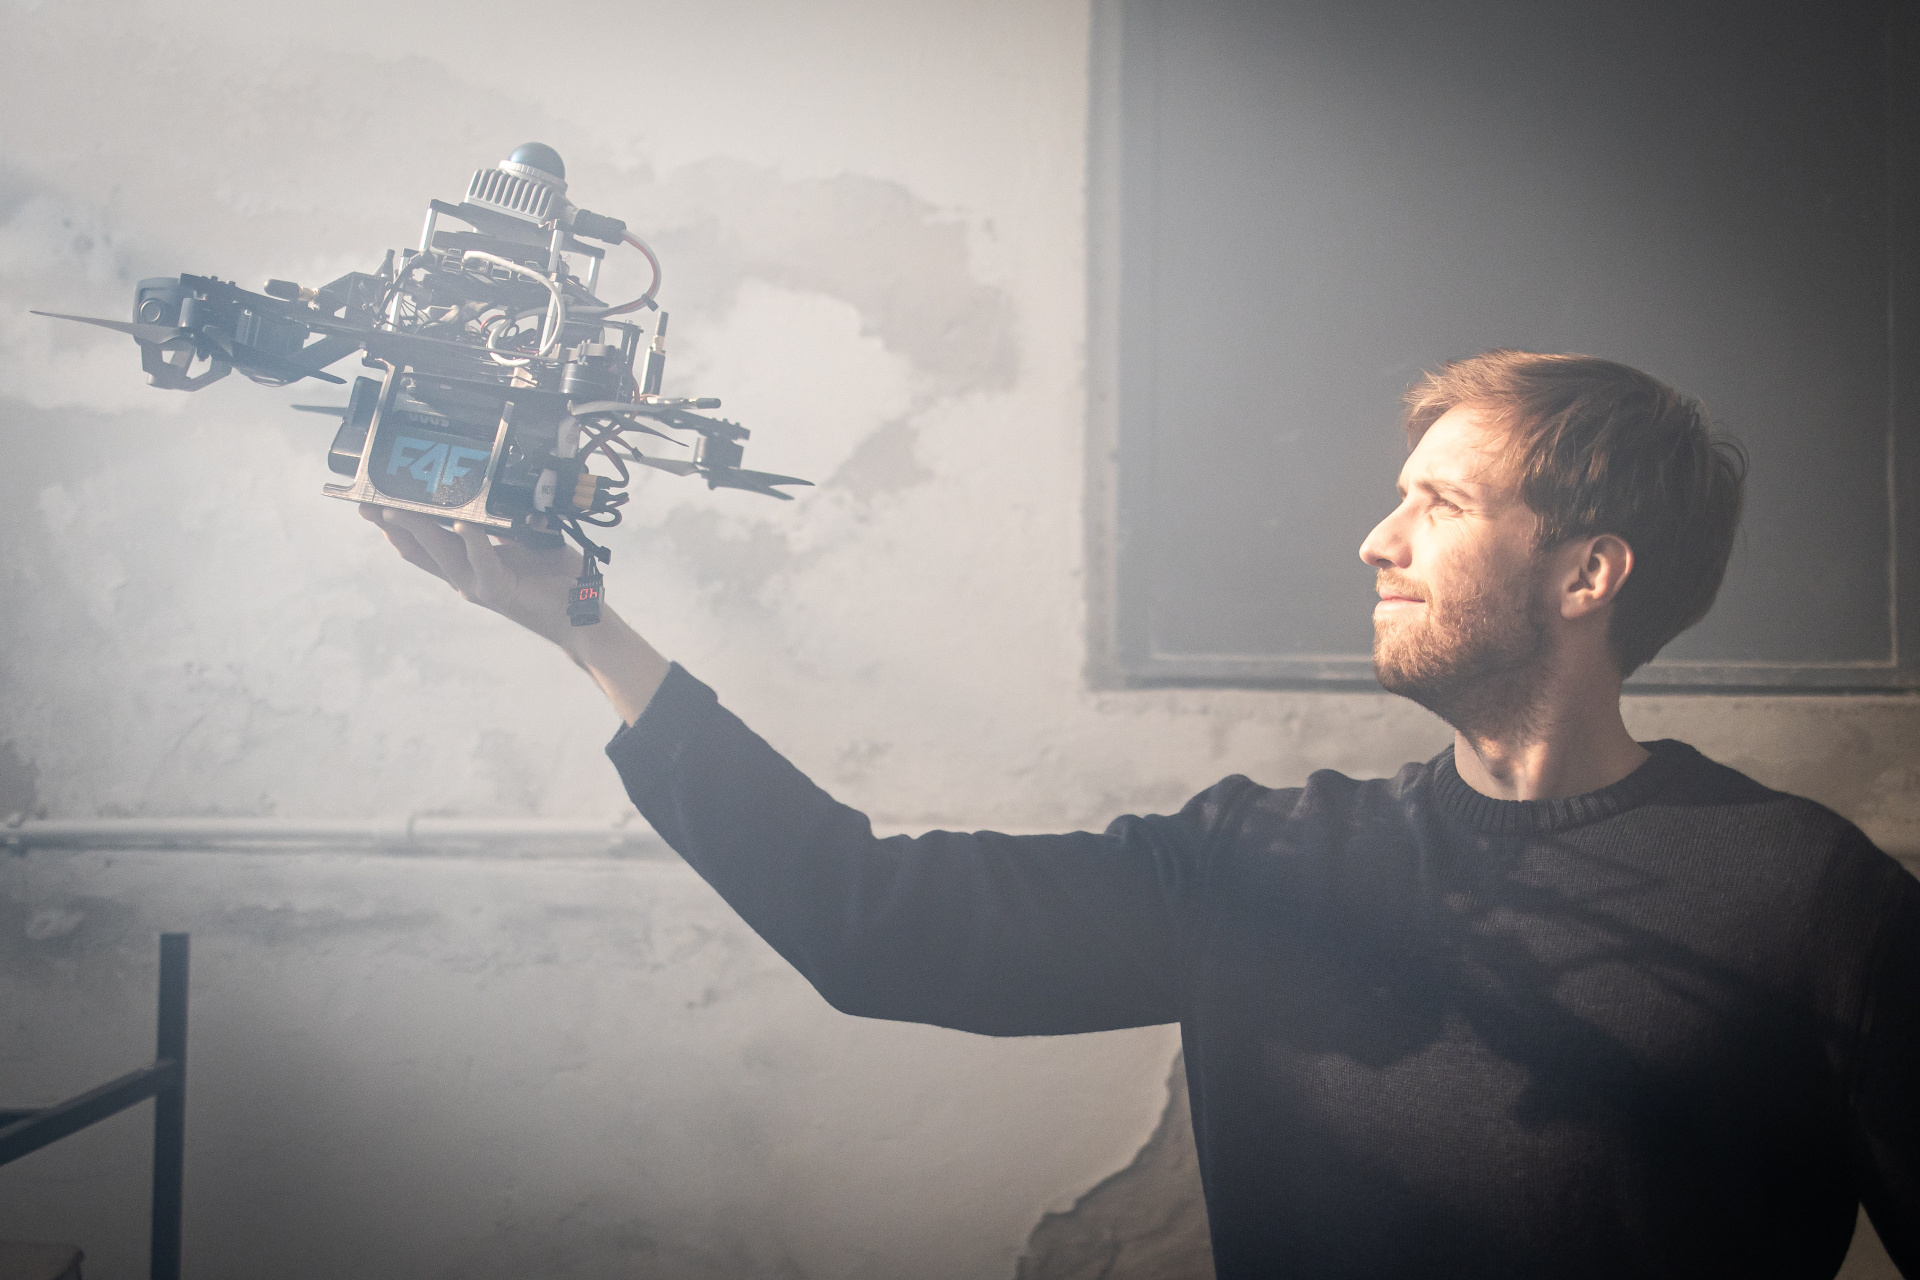
\includegraphics[width=7.0cm]{fig/profile.jpg}\\

\vspace{-1.5cm}
\section*{}
\Large \textbf{Pavel Petráček}
\vspace{2mm}\\
\normalsize \textbf{PhD} in Autonomous Robotics
\vspace{2mm}\\
\normalsize Robotics R\&D Lead @ Fly4Future
\normalsize Researcher @ Multi-Robot Systems
% \end{center}

\vspace{5mm}
% \section*{Contact}
\begin{itemize}
\item \faLocationArrow~ Prague, Czech Republic
\item \faPhone~ +420 739 757 519
\item \faEnvelope~ \Colorhref{mailto:petracekpav@gmail.com}{petracekpav@gmail.com}
\item \faHome~ \Colorhref{https://mrs.fel.cvut.cz/pavel-petracek}{mrs.fel.cvut.cz/pavel-petracek}
\item \faGithub~ \Colorhref{https://github.com/petrapa6}{github.com/petrapa6}
\item \faLinkedin~ \Colorhref{https://www.linkedin.com/in/pavelpetracek/}{linkedin.com/pavelpetracek}
\item \faStickyNote~ \Colorhref{https://raw.githubusercontent.com/petrapa6/cv/master/academic_cv.pdf}{Link} to academic CV
\item \faGoogle~ \Colorhref{https://scholar.google.com/citations?user=IwzN6MQAAAAJ}{Google Scholar}
\end{itemize}

\vspace{0.6em}
\section*{About me}
% Robotics R\&D engineer and team lead with 10 years of experience in autonomous small-aircraft systems and field-tested robotics. Delivered robust UAV systems for cultural heritage and disaster response.
Robotics R\&D engineer and team lead with 10 years of hands-on experience in autonomous UAV systems, multi-robot coordination, and robotics for real-world applications.
Experienced in taking research from concept to deployment in high-impact environments like subterranean S\&R and heritage preservation.
Technical expert with strong academic background and project leadership.

\vspace{0.4em}
\noindent

\vspace{0.4em}
\noindent
Fast learner open to new things.

\vspace{0.6em}
\section*{Core skills}
GNSS-denied robot autonomy\\
SLAM, 3D mapping, perception\\
Embedded systems, sensor fusion\\
Real-time system integration
\begin{itemize}[label=\whitesquare, left=1.0em]
  \item C++, Python, ROS, PX4, git
\end{itemize}
Multi-agent systems\\
Technical and R\&D leadership

\vspace{0.6em}
\section*{Languages}
Czech (native)\\
English (fluent)

\switchcolumn

% === RIGHT COLUMN ===
\color{primary}

\vspace{-0.5cm}
\section*{Experience}

\textbf{Fly4Future s.r.o.} \hfill \textit{2023–Present} \\
R\&D Projects Lead \& Developer
\begin{itemize}[label=\bluesquare, left=0.5em]
  \item Leading robotics R\&D team of 6 in solving real-world challenges
  \item Hands-on approach to development and experimentation
\end{itemize}

\vspace{0.35cm}
\noindent
\textbf{Multi-Robot Systems @ CTU} \hfill \textit{2016–Present} \\
Researcher \& Developer
\begin{itemize}[label=\bluesquare, left=0.5em]
  \item Fundamental research and its transfer to practice
  % \item Leading R\&D projects
  \item Projects leadership, students mentoring, international cooperation, public demos, teaching
  \item Open-source contributor (\Colorhreff{https://github.com/ctu-mrs/mrs_uav_system}{\textbf{MRS UAV System}})
  % \item Key contributor to DARPA SubT Challenge — GNSS-denied UAV autonomy.
\end{itemize}

\vspace{0.35cm}
\noindent
\textbf{CertiCon a.s.} \hfill \textit{2016–2017} \\
Software Tester
\begin{itemize}[label=\bluesquare, left=0.5em]
  \item Learned corporate workflows \& developed automated tests
\end{itemize}

\section*{Selected projects}

\noindent
\textbf{DARPA Subterranean Challenge} (\Colorhreff{http://mrs.fel.cvut.cz/projects/darpa}{\textbf{link}})
\begin{itemize}[label=\bluesquare, left=0.5em]
  \item Subterranean search \& rescue with autonomous robot teams
  \item Responsible for system design, GNSS-denied autonomy, mapping, SLAM, experimentation, integration, and deployment of UAVs
  \item Winning \$1M while competing with \Colorhreff{https://spectrum.ieee.org/darpa-subterranean-challenge}{top world institutions} 
\end{itemize}

\vspace{0.2cm}
\noindent
\textbf{Dronument} (\Colorhreff{https://www.youtube.com/watch?v=Gx-mBklSbYc}{\textbf{video}})
\begin{itemize}[label=\bluesquare, left=0.5em]
    \item Documenting interiors of historical monuments with multiple cooperating UAVs in a synchronized multi-robot formation
    \item Achieved reliable operation and deployed the autonomous system in 20 historical sites (incl. 2 UNESCO sites)
\end{itemize}

\vspace{0.2cm}
\noindent
\textbf{Multi-UAV swarming} (\Colorhreff{https://www.youtube.com/watch?v=Ax3ONfo1hMA}{\textbf{video}})
\begin{itemize}[label=\bluesquare, left=0.5em]
    \item Deployed first fully-decentralized swarms w/o communication
\end{itemize}

\vspace{0.2cm}
\noindent
\textbf{DOFEC} (\Colorhreff{https://www.youtube.com/watch?v=QHpifXJzH5g}{\textbf{video}})
\begin{itemize}[label=\bluesquare, left=0.5em]
    \item Designed onboard fire detection \& localization with autonomous mission execution and fire extinguishment
\end{itemize}

\section*{Education}
\textbf{PhD, Autonomous Flying Robotics} \hfill CTU, 2019-2024
\begin{itemize}[label=\bluesquare, left=0.5em]
  \item Topic: UAV autonomy in perception-degraded settings (\Colorhreff{https://mrs.fel.cvut.cz/data/papers/petracek_phd_thesis.pdf}{\textbf{pdf}})
  \item Numbers: 19 publications; h-index 9 (WoS), 15 (GScholar)
\end{itemize}

\vspace{0.2cm}
\noindent
\textbf{BSc \& MSc, Cybernetics} \hfill CTU, 2014-2019

\section*{Honors \& Awards}
\textbf{Werner von Siemens prize} (\Colorhreff{https://www.cenasiemens.cz/minule-rocniky/vitezove-2024/\#disertacni-prace}{\textbf{web}}, \Colorhreff{https://www.youtube.com/watch?v=idnDA4Ap-J4}{\textbf{video}}) \hfill 2025
\begin{itemize}
  \item \#1 dissertation out of top (243) 2023-2024 STEM works in Czechia
\end{itemize}

\vspace{0.2cm}
\noindent
\textbf{Joseph Fourier prize} (\Colorhreff{https://feedit.cz/2025/06/26/vymyslel-zpusob-jak-mohou-drony-letat-uvnitr-budov-mlady-cesky-vedec-za-to-ziskal-cenu-josepha-fouriera-a-staz-ve-francii/}{\textbf{web}} in Czech) \hfill 2025
\begin{itemize}
  \item \#1 dissertation out of top (65) 2024 CS works in Czechia
\end{itemize}

\vspace{0.2cm}
\noindent
\textbf{Best paper award at IEEE RA-M} (\Colorhreff{https://www.linkedin.com/posts/mrsgroupprague_icra2025-robotics-dronetechnology-activity-7332784284316962816-kg45}{\textbf{web}}, \Colorhreff{https://mrs.fel.cvut.cz/data/papers/petracek2023ram.pdf}{\textbf{paper}}) \hfill 2025
\begin{itemize}
  \item Robotics \& Automation Magazine award for our \Colorhreff{https://www.youtube.com/watch?v=Gx-mBklSbYc}{\textbf{Dronument}} work
\end{itemize}

\vspace{0.2cm}
\noindent
\textbf{Dean's prize} (\Colorhreff{https://cyber.felk.cvut.cz/news/pavel-petracek-received-the-deans-award-for-prestigious-dissertation/}{\textbf{link}}) \hfill 2024, 2019, 2017
\begin{itemize}
  \item All my theses (dissertation, master's \& bachelor's) were selected in top 1\% works at FEE CTU in their respective category and year
\end{itemize}

\vspace{0.2cm}
\noindent
\textbf{Czech National Excellence Award M17+} \hfill 2022
\begin{itemize}
  \item Excellent international evaluation of our Dronument solution (\Colorhreff{https://mrs.fel.cvut.cz/dg18p02ovv069-fvz}{\textbf{link}})
\end{itemize}

% \vspace{0.2cm}
% \noindent
% \textbf{Dean's prize} \hfill 2017, 2019
% \begin{itemize}
%   \item BSc and MSc theses selected in top 1\% at FEE CTU
% \end{itemize}

\end{paracol}

\end{document}
